\documentclass{ujarticle}
\usepackage{robomech2022}
\usepackage[dvipdfmx]{graphicx}
\usepackage{url}
\usepackage{caption}
\captionsetup[table]{justification=centering}
\captionsetup[figure]{justification=centering}


\begin{document}
\makeatletter
\title{視覚と行動のend-to-end学習による経路追従行動の模倣}
{―データセットを収集してオフラインで訓練する手法の検討―}
{A proposal for imitation method of path-tracking behavior by end-to-end\\ learning of vision and action}
{-Validation of a method to collect and train dataset offline-}

\author{
\begin{tabular}{lll}
 \hspace{1zw}○学\hspace{1zw}髙橋祐樹(千葉工大) & \hspace{1zw} \hspace{2zw}白須和暉(千葉工大) & \hspace{-6.5zw} 学\hspace{1zw}藤原柾(千葉工大) \\
 \hspace{2zw}正\hspace{1zw}上田隆一(千葉工大) & \hspace{1zw} 正\hspace{1zw}林原靖男(千葉工大)\\
 % ※協賛・後援団体の会員資格で発表される場合は「正・学」は不要です。
 &\\
 \multicolumn{2}{l}{\small Yuuki TAKAHASHI, Chiba Institute of Technology, s19c1068aq@s.chibakoudai.jp}\\
 \multicolumn{2}{l}{\small Kazuki SHIRASU, Masaki FUJIWARA, }\\
 \multicolumn{2}{l}{\small Ryuichi UEDA and Yasuo HYASHIBARA, Chiba Institute of Technology}\\
\end{tabular}
}
\makeatother

\abstract{ \small 
In this paper, we propose a method of training a robot by collecting data on and near a target path, based on a conventional method of imitation learning. In the proposed method, the robot is placed on and around the target path and data is collected. Then, the robot is trained off-line using the collected data. After learning, the robot runs according to the output of the trainer using camera images as input. This is performed on a simulator, and the effectiveness of the proposed method is verified through experiments. As a result, it is confirmed that the proposed method can run around the path.
}

\date{} % 日付を出力しない
\keywords{End-to-End Learning, Navigation, Offline}

\maketitle
\thispagestyle{empty}
\pagestyle{empty}

\small
\section{緒言}%===========================
本研究グループでは, end-to-end学習により, 視覚に基づく経路追従行動をオンラインで生成する手法の提案を行い, その有効性を実験により検証してきた\cite{si2020-okada}\cite{si2021-okada}. 視覚を入力として, end-to-end学習により経路追従行動を模倣する手法はいくつか提案されている. 例えば, Bojarskiらは, 人が操作するステアリングの角度をend-to-end学習することで経路追従する手法を提案した\cite{bojarski}. Jing Biらは, 歩行者が多い環境における経路追従行動の模倣に取り組んでいる\cite{pedestrian}. それに対して, 本研究グループでは, 図1に示すように, 測域センサなどを入力として自己位置推定を行い生成した行動を, カメラ画像を入力とする行動に模倣する手法を提案している. この手法は, 多くの研究\cite{bojarski}\cite{pedestrian}が人の操作を模倣していたのに対して, 自動制御の出力を模倣する点に特徴がある. \par しかし, 岡田らの手法(以下「従来手法」と称する)では, データ収集及び学習を行う際にロボットを走らせるため, 時間が必要となる. \par そこで, 本研究では従来手法を基にロボットを走らせることなく, 目標経路上及びその周辺のデータを一度に収集してオフラインで訓練する手法を提案する. これにより, 訓練に要する時間を短縮できることが期待できる. さらに訓練後に, カメラ画像を入力とした学習器の出力で自律走行させることで手法の有効性を検証することを目的とする. \par また, 本研究の手法を実ロボットに適用する際には, ロボットの進行方向に対して平行な方向にカメラを取り付けることで再現する. その際に, カメラがどの程度あれば経路追従が可能であるかをシミュレータ上の実験により確認する. 
% また, 清岡ら\cite{si2021-kiyooka}により, 経路から離れた状態も訓練データに加えた方が, 経路から離れても再び経路に戻る可能性が高いことが示されている.

\begin{figure}[h]
	\centering
	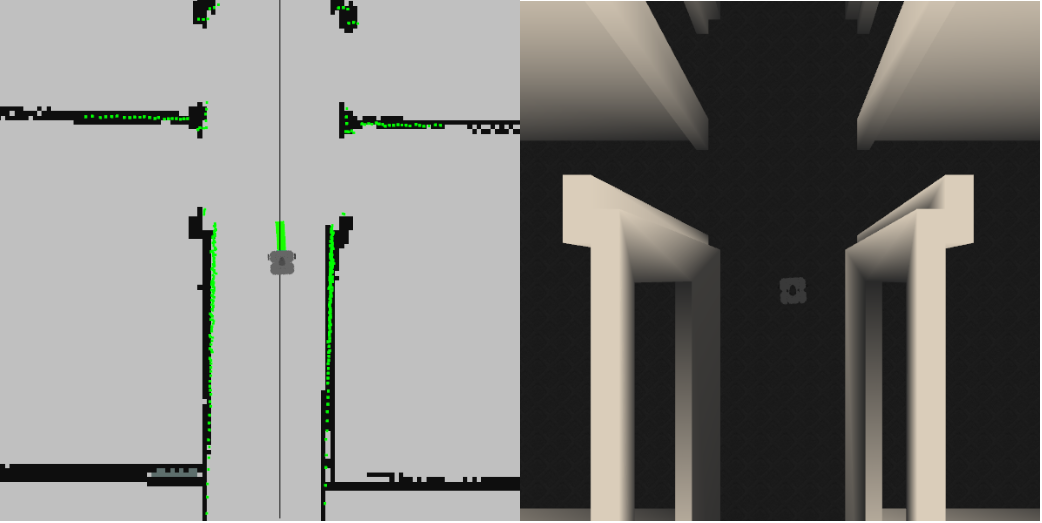
\includegraphics[width=0.416\textwidth]{img/navigation.png}
	\caption{Moving with map-based navigation}
	\label{Fig:navigation}
\end{figure}

\newpage
\section{従来手法}%===========================
従来手法に関して述べる. 従来手法では, 地図を用いたルールベース制御器の出力を模倣し, 経路追従行動を獲得する. 図\ref{Fig:si2020-okada}に示すシステムでは, 学習時に測域センサとオドメトリを入力としたnavigation\cite{navigation}の出力である角速度(以下「目標角速度」と称する)を学習器とモータ駆動系に与える. 学習器には, カメラ画像を64×48にリサイズした3つのカメラ画像(RGB画像)を入力し,目標角速度を出力してend-to-end学習する. 左右のカメラ画像に対する角速度には, それぞれ経路に戻るようなオフセットを加える. 訓練後は, 図\ref{Fig:si2020-okada-test}のようにカメラ画像を入力とした学習器の出力により走行する. なお, テストフェーズでは3台のカメラのうち, 中央のカメラのみ使用する. \par また, 従来手法で用いたネットワークの構造を図\ref{Fig:cnn}に示す. 構造は入力層1, 畳み込み層3, 全結合層2, 出力層1の全7層から構成されている. また, オンラインで学習が行えるように, ネットワークは畳み込みニューラルネットワーク(CNN)を元にしている. 

\begin{figure}[h]
		\centering
		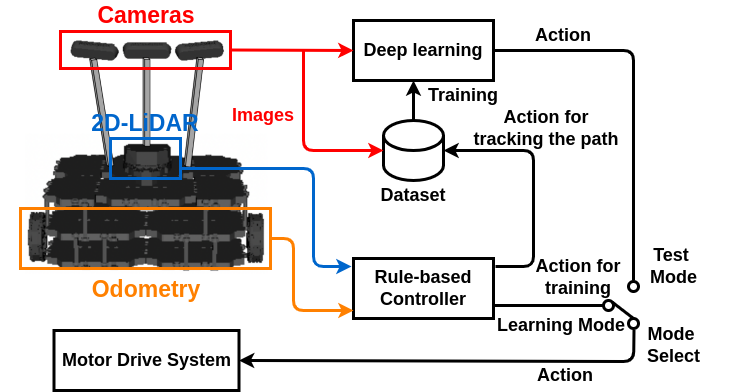
\includegraphics[width=0.5\textwidth]{img/si2020-okada.png}
		\caption{Learning phase}
		\label{Fig:si2020-okada}
\end{figure}

\begin{figure}[h]
	\centering
	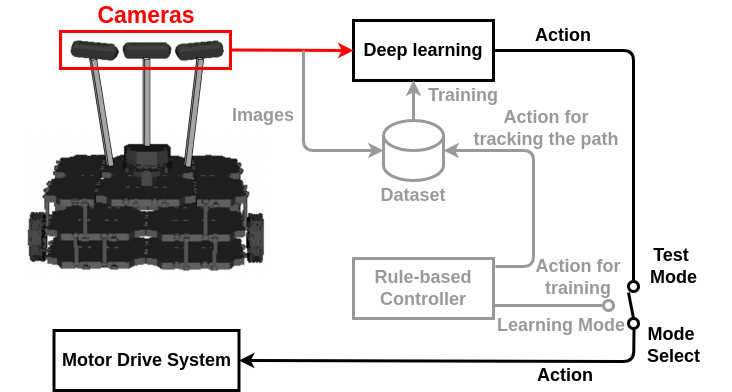
\includegraphics[width=0.5\textwidth]{img/si2020-okada-test.png}
	\caption{Test phase}
	\label{Fig:si2020-okada-test}
\end{figure}

\begin{figure}[h]
	\centering
	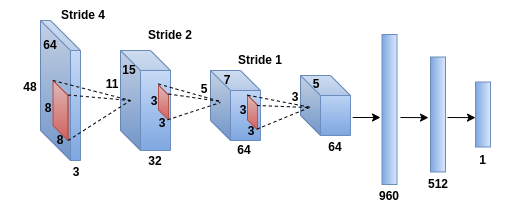
\includegraphics[width=0.45\textwidth]{img/cnn.png}
	\caption{Structure of network}
	\label{Fig:cnn}
\end{figure}

\newpage
\section{提案手法}%===========================
本研究で提案する手法を述べる. 従来手法に対して, 提案手法は一度にデータを収集して, オフラインで訓練することが異なる. 図\ref{Fig:collect}にデータの収集方法を示す. 赤線の目標経路から平行に離れた座標にロボットを配置する. ロボットの進行方向に対する並進速度は0m/sであるが, 目標角速度はロボットに与えられる. そして, その座標ごとに64×48のカメラ画像(RGB画像)と目標角速度を図のように収集する. このように, ロボットを走行させることなく, 目標経路上及びその周辺に配置することで, 一度に大量のデータを収集することができる. その後, 収集したデータを用いてオフラインで学習を行う.

\begin{figure}[h]
		\centering
		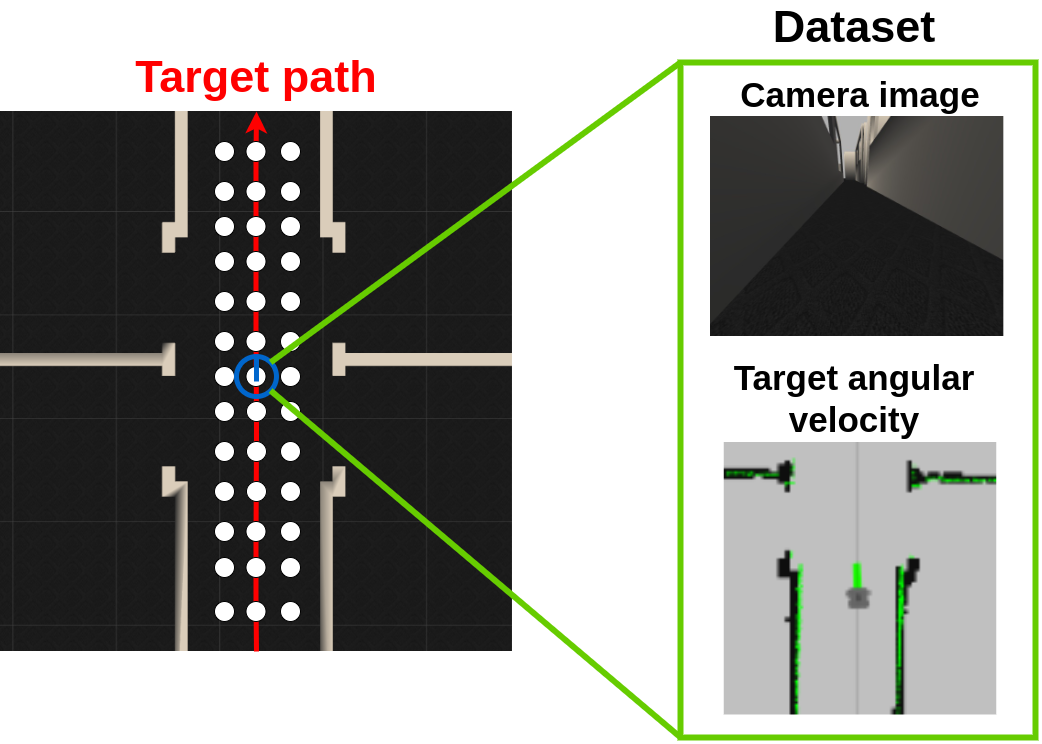
\includegraphics[width=0.45\textwidth]{img/proposed.png}
		\caption{Method of collecting data around the target path}
		\label{Fig:collect}
\end{figure}

\section{シミュレータを用いた実験}%=========================== 
\subsection{実験装置}シミュレータにはGazebo\cite{gazebo}のWillow Garage\cite{willow}を用いて, 図\ref{Fig:willow}に示すコースで行う. また, ロボットモデルにはカメラを3つ搭載したTurtlebo3 Waffle Pi\cite{turtlebot3}を用いた. 

\begin{figure}[h]
		\centering
		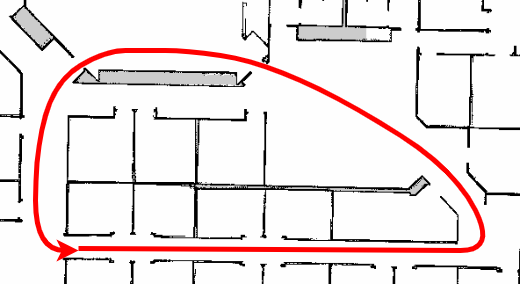
\includegraphics[width=0.4\textwidth]{img/willow-path.png}
		\caption{Course to collect data}
		\label{Fig:willow}
\end{figure}

\newpage
\subsection{実験方法}
\begin{description}
		\item[1.データ収集フェーズ]図\ref{Fig:collect-data}にデータの収集方法を示す. データ収集フェーズでは, 従来手法と同様に3台のカメラを使用する. 実験1では, 赤線の目標経路上のみにロボットを配置する. 実験2では, 目標経路上には配置せずに, 経路から平行に±0.1[m]離れた座標に配置する. そして, 実験3と実験4では, 目標経路上と経路から平行に±0.1[m]離れた座標にロボットを配置する. ただし, 実験1から実験4のロボットの進行方向の配置間隔は0.1[m]とする. そして, その座標ごとに経路に沿った向きを基準として±5度傾けて, カメラ画像と目標角速度を収集する. 
		\item[2.訓練フェーズ]従来手法では, オンラインで学習を行うため, 計算のリソースなどの観点などからミニバッチ学習を用いていた. しかし, 本手法はオフラインで学習を行うため, バッチ学習を用いる. 実験1から実験3は4000step, 実験4は2000step学習した. なお, 4000stepは従来手法において, シミュレータの実験に用いられてきたステップ数である. 
		\item[3.テストフェーズ]図\ref{Fig:willow}に示したコースで10個の学習済みモデルを用いて走行させる. 経路を3周できた場合を成功とし, 壁に衝突したり, 目標経路から10[m]以上離れたりした場合を失敗とした. また, 並進速度は0.2[m/s]で一定の速度をロボットに与える. ただし, テストフェーズでは従来手法と同様に3台のうち, 中央のカメラのみを使用する. 
\end{description}

\begin{figure}[h]
		\centering
		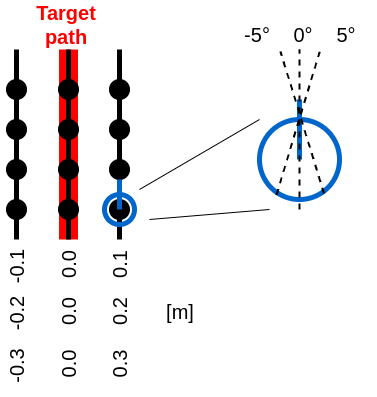
\includegraphics[width=0.45\textwidth]{img/collect2.png}
		\caption{Method of collecting data around the target route}
		\label{Fig:collect-data}
\end{figure}

\newpage
\subsection{実験結果と考察}実験結果を表\ref{tb:result}に示す. 実験1では, 角を曲がりきれずにコースアウトすることがほとんどであった. これは, 直進時の行動を学習する割合が実験2から実験4と比べて多く, 左折するデータが少ないためだと考えられる. 実験2では, 経路上のデータのみがないため, 直進時にふらつきながら走行する様子が多く見られた. 実験4は, 実験3の半分のステップ数でも成功回数があまり変わらなかった. ここで, 学習時のlossの一例を図\ref{Fig:loss}に示す. 図から実験1は, オーバフィッティングしていると考えられる. また, 実験2から実験4は学習が収束している様子が確認できる. これらのことから, 学習時に経路上及びその周辺のデータを用いる方が, 経路追従できる可能性が高いと考えられる. また, 学習時に経路上のデータを用いなくても, 概ね成功回数は変わらないことも確認できた. 因みに, 従来手法が訓練に最低40分程度必要であったのに対して, 実験3は訓練時間が4分程度であるため, 大幅に時間を短縮できることを確認した. 

\begin{table}[h]
		\caption{Number of successes in the experiment}
		\centering
		\scalebox{1.0}{
		\begin{tabular}{|c|c|} \hline
			Experiments & Number of successes \\ \hline
			Exp.1(4000step) & 0/10 \\ \hline
			Exp.2(4000step) & 9/10 \\ \hline
			Exp.3(4000step) & 10/10 \\ \hline
			Exp.4(2000step) & 9/10 \\ \hline
		\end{tabular}
		}
		\label{tb:result}
	\end{table}

\begin{figure}[h]
		\centering
		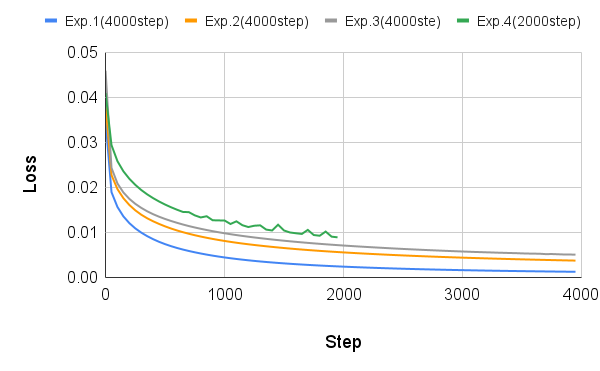
\includegraphics[width=0.5\textwidth]{img/loss_compe_fix.png}
		\caption{Loss value in the experiments}
		\label{Fig:loss}
\end{figure}

\section{結言}%===========================
本稿では, 従来手法を基にロボットを走行させることなく目標経路及びその周辺のデータを一度に収集して, オフラインで訓練する手法を提案した. 実験では, 訓練時に経路上だけでなく, 経路周辺のデータも訓練データに加えた方が経路追従できる可能性が高いことを確認し, 手法の有効性を示した. また, 従来手法と比べて訓練時間を大幅に短縮できることを確認した. 


\footnotesize
\begin{thebibliography}{99}

\bibitem{si2020-okada}
岡田 眞也, 清岡 優祐, 上田 隆一, 林原 靖男: ``視覚と行動のend-to-end学習により経路追従行動をオンラインで模倣する手法の提案'', \textit{計測自動制御学会 SI 部門講演会 SICE-SI2021 予稿集}, pp.1147-1152, 2020.

\bibitem{si2021-okada}
岡田 眞也, 清岡 優祐, 春山 健太, 上田 隆一, 林原 靖男: ``視覚と行動のend-to-end学習により経路追従行動をオンラインで模倣する手法の提案-“経路追従行動の修正のためにデータセットを動的に追加する手法の検討'', \textit{計測自動制御学会 SI 部門講演会 SICE-SI2021 予稿集}, pp.1066-1070, 2021.	

\bibitem{bojarski}
Bojarsi, Mariusz, et al.:``End to End Learning for Self-Driving Cars.'', arXiv: 1604.07316, 2016

\bibitem{pedestrian}
Jing Bi, Tianyou Xiao, Qiuyue Sun, Chenliang Xu. ``Navigation by Imitation in a Pedestrian-Rich Environment'', 	arXiv:1811.00506, 2018

% \bibitem{si2021-kiyooka}
% 清岡 優祐, 岡田 眞也, 岩井 一輝, 上田 隆一, 林原 靖男: ``視覚と行動のend-to-end学習により経路追従行動をオンラインで模倣する手法の提案''-データセットと生成された経路追従行動の解析'', \textit{計測自動制御学会 SI 部門講演会 SICE-SI2021 予稿集}, pp.1072-1075, 2021.

\bibitem{navigation}
ros-planning, navigation リポジトリ\\
\url{https://github.com/ros-planning/navigation}\\
(最終閲覧日 \today)

\bibitem{gazebo}
gazebo リポジトリ\\
\url{http://gazebosim.org/}\\
(最終閲覧日 \today)

\bibitem{willow}
Koenig, Nathan, and Andrew Howard. ”design and use paradigms for gazebo, an open-source multi-robot simulator.”. 2004 IEEE/RSJ International Conference on Intelligent Robots and Systems (IROS)(IEEE Cat. No. 04CH37566). Vol. 3. IEEE, pp.2149-2154(2004).\\
(最終閲覧日 \today)

\bibitem{turtlebot3}
Turtlebot3-robotis emanual.robotis.\\
\url{https://emanual.robotis.com/docs/.}\\
(最終閲覧日 \today)

\end{thebibliography}

\normalsize
\end{document}
